\documentclass{article}
\usepackage{physics}
\usepackage{amsmath}
\usepackage{hyperref}
\usepackage{graphicx}
\title{Modelling COVID-19 pandemic using SIS Model}
\author{Lashit Jain - 201402162 \\ Ayush Tripathi - 201202159}
\begin{document}
	\maketitle
	\section{Introduction}
	\subsection{Background}
	Coronaviruses are enveloped RNA viruses that cause respiratory illnesses of varying severity from the common cold to fatal pneumonia. Numerous coronaviruses, first discovered in domestic poultry in the 1930s, cause respiratory, gastrointestinal, liver, and neurologic diseases in animals. Only 7 coronaviruses are known to cause disease in humans.

	Three of the 7 coronaviruses cause much more severe, and sometimes fatal, respiratory infections in humans than other coronaviruses and have caused major outbreaks of deadly pneumonia in the 21st century:
	\begin{enumerate}
	\item SARS-CoV2 is a novel coronavirus identified as the cause of coronavirus disease 2019 (COVID-19) that began in Wuhan, China in late 2019 and spread worldwide.
	\item MERS-CoV was identified in 2012 as the cause of Middle East respiratory syndrome (MERS). 
	\item SARS-CoV was identified in 2002 as the cause of an outbreak of severe acute respiratory syndrome (SARS).
	\end{enumerate}

	COVID-19, meanwhile, is a `novel' coronavirus, meaning it is a new strain and has not been previously identified in humans. 

	\subsection{Transmission of COVID-19}
	COVID-19 spreads mainly by droplets produced as a result of coughing or sneezing of a COVID-19 infected person. This can happen in two ways: 
	\begin{itemize}
	\item \textit{Direct close contact:} One can get the infection by being in close contact with COVID-19 patients (within one meter of the infected person), especially if they do not cover their face when coughing or sneezing.
	\item \textit{Indirect contact:} The droplets survive on surfaces and clothes for many days. Therefore, touching any such infected surface or cloth and then touching one’s mouth, nose or eyes can transmit the disease.
	\end{itemize}

	\subsection{Epidemiological models}
	Kermack and McKendrick in 1927[1] laid the foundation for two very important models in the field of epidemiology:
	\begin{itemize}
		\item SIS Model: This is used to model diseases that do not confer with immunity. It stands for Susceptible Infectious Susceptible. In it a person is first susceptible, then gets infected and after infection is gone, becomes susceptible again.
		\item SIR Model: This is used to model diseases in which one can get recovered from the disease by developing immunity. It stands for Susceptible Infectious Recovered. In it a person is first susceptible, then gets infected and after infection is gone, becomes recovered. Recovered patients do not catch infection again.
	\end{itemize}

	\subsection{Motivation}
	Most of the models that are being proposed recently for COVID-19 are based on SIR models[4]. However recent reports show that recovered patient might get the infection back[3,5]. This calls for exploring the possibility of COVID-19 not being fully conferred by immunity. 

	Our plan is to model the COVID-19 spread using the SIS model. We propose two models SISD and SIXD to model the pandemic. To the best of our knowledge, there exists no study which determines COVID-19 spread using the SIS model.

	
	\section{SISD}
	While deploying SIS model for COVID-19, we quickly realised the need for another parameter for death. Hence we extended the basic model to SISD. Here a infected patients can either go to Susceptible state or Dead State. This model assumes that COVID-19 does not confer with immunity at all.
	\begin{equation*}
		\dv{s}{t} = -\beta si + \alpha i
	\end{equation*}
	\begin{equation*}
		\dv{i}{t} = \beta si - \alpha i - \gamma i
	\end{equation*}
	\begin{equation*}
		\dv{d}{t} = \gamma i
	\end{equation*}
	where $\gamma$ represents mortality rate, $\beta$ represents transmission rate and $\alpha$ represents rate of true recovery (not dying). $s, i, d$ are normalised paramters.


	\section{SIXD}
	The above model has serious shortcomings. Even though COVID-19 \textit{re-occurs}, there is clear evidence that antibodies develop against the virus. Though we're not sure about their effectiveness and why the reoccurence occurs. However, it can mainly be due to two factors:
	\begin{itemize}
		\item \textbf{Re-infection:} The patients that have recovered are catching the infection again. WHO has warned not to rule out this possibility but we do not have any strong evidence that this is the case. Also, we do not have any idea about the behaviour of re-infection and hence we do not model it in this current report.
		\item \textbf{Re-activation:} The virus is re-activating in patients after they have recovered. There has been evidence for this behaviour and it is being assumed it can occur due to one of the two reasons:
		\begin{itemize}
		\item The virus lies in dormant state in the body and is reactivated again.
		\item The testing kits are not very accurate.
		\end{itemize}
		We chose to model the first scenario but we will ignore the case of recovered patients being re-infected again as we don't have enough evidence to map it's behaviour. Therefore we present SIXD model, in which a person can go from infectious to ex-infectious or dead state. The ex-infectious can come back to infectious state with a reactivation rate.
	\end{itemize}

	\subsection{Reactivation Case: Dormant virus}
	\begin{equation*}
		\dv{s}{t} = -\beta si
	\end{equation*}
	\begin{equation*}
		\dv{i}{t} = \beta si - \alpha i - \gamma i + \theta x
	\end{equation*}
	\begin{equation*}
		\dv{d}{t} = \gamma i
	\end{equation*}
	\begin{equation*}
		\dv{x}{t} = \alpha i -\theta x
	\end{equation*}
	where $\gamma$ represents mortality rate, $\beta$ represents transmission rate, $\alpha$ represents rate of true recovery (not dying) and $\theta$ represents reactivation rate (per ex-infected person).
	\newpage

	\section{Method}
	\subsection{Parameters}
	We obtained rate data from the MIDAS Research Network[2]. It is summarised in the following table:
	\begin{center}
		\begin{tabular}{ |c|c| } 
		 \hline
		 & \\
		 \hline
		 Basic Reproduction Rate & 4.0 \\ 
		 \hline
		 Recovery time & 21.02 \\ 
		 \hline
		\end{tabular}
	\end{center}

	Above data helped us in approximating the parameter values:
	\begin{center}
		\begin{tabular}{ |c|c| } 
		 \hline
		 Transmission Rate & 0.2 \\ 
		 \hline
		 Recovery Rate & 0.05 \\
		 \hline
		 Mortality Ratio & 0.02\\ 
		 \hline
		\end{tabular}
	\end{center}

	Note that above Recovery Rate is for SIR models in which death is also included as recovery. We can use mortality ratio to get our paramters.


	For calculating the reactivation rate ($\theta$) we obtained reactivation data for three datas from the Korean CDC[3].
	\begin{center}
		\begin{tabular}{ |c|c|c|c|c| } 
		 \hline
		  & Recovered & Reactivated & Ratio & Normalised (per 1000) \\ 
		 \hline
		 09/04/2020 & 6973 & 91 & 0.013 & 13 \\ 
		 \hline
		 12/04/2020 & 7368 & 116 & 0.016 & 16\\ 
		 \hline
		 26/04/2020 & 8764 & 222 & 0.025 & 25\\
		 \hline
		\end{tabular}
	\end{center}

	We can calculate $\theta$ by taking the average of the mutual slopes of three points above:
	\begin{equation*}
		\theta = \frac{\frac{16-13}{12-9} + \frac{25-16}{26-12} + \frac{25-13}{26-3}}{3*1000} = 0.00085
	\end{equation*}
	
	\subsection{Social Distancing}
	To incorporate social distancing in the above equations, we multiply $\beta$ in above equations by a factor $\rho$. $\rho = 0.4$ implies a social distancing with $60\%$ effectiveness.


	\subsection{Software}
	We simulated above equations using python libraries which include Matplotlib and NumPy.

	\newpage

	\section{Results}
	
	\subsection{SISD}
	\begin{figure}[h!]
		\centering
		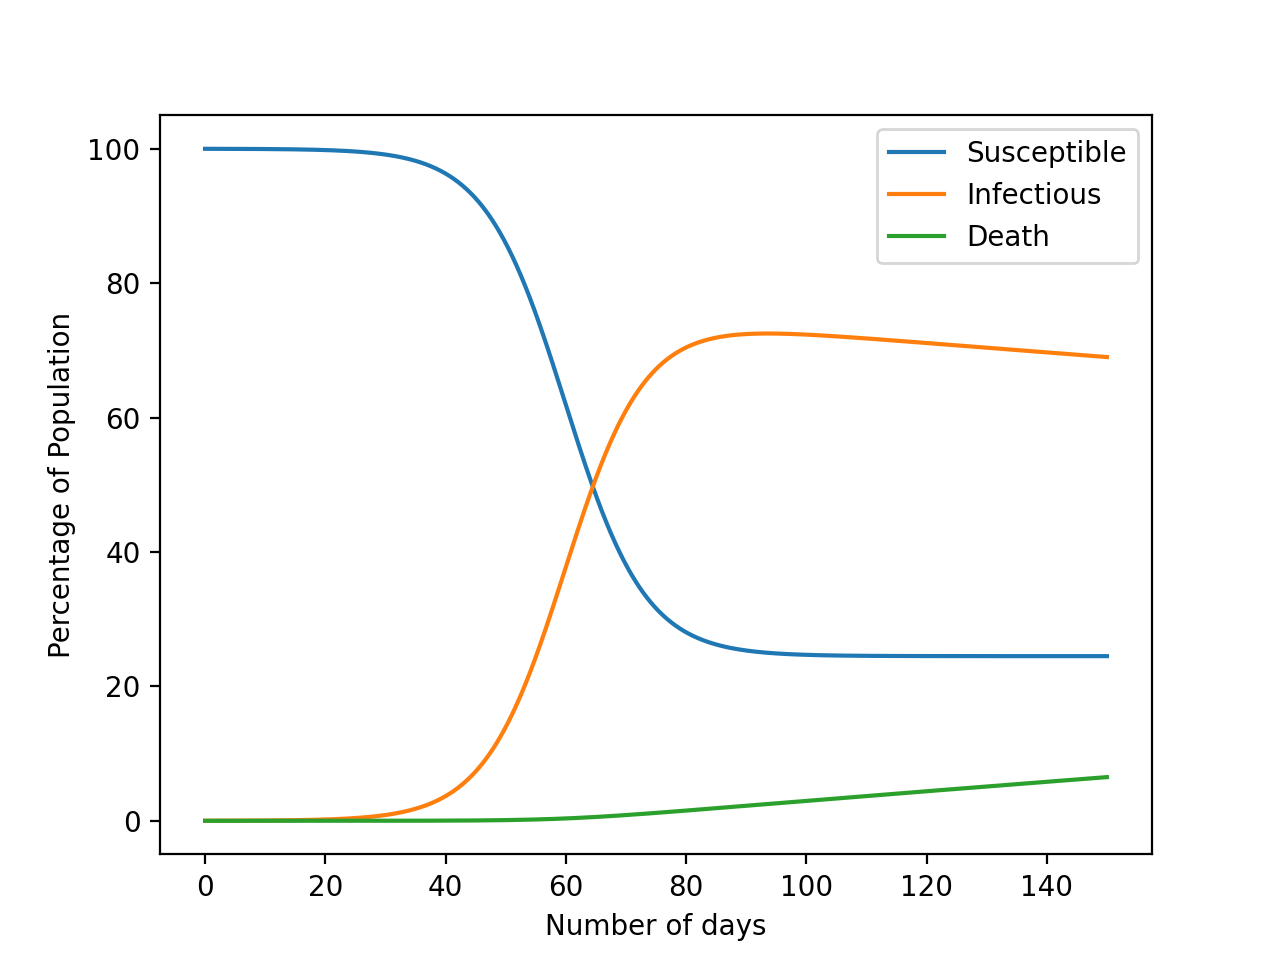
\includegraphics[width=90mm]{images/SISD/standard.png}
		\caption{SISD}
	\end{figure}
	\begin{figure}[h!]
		\centering
		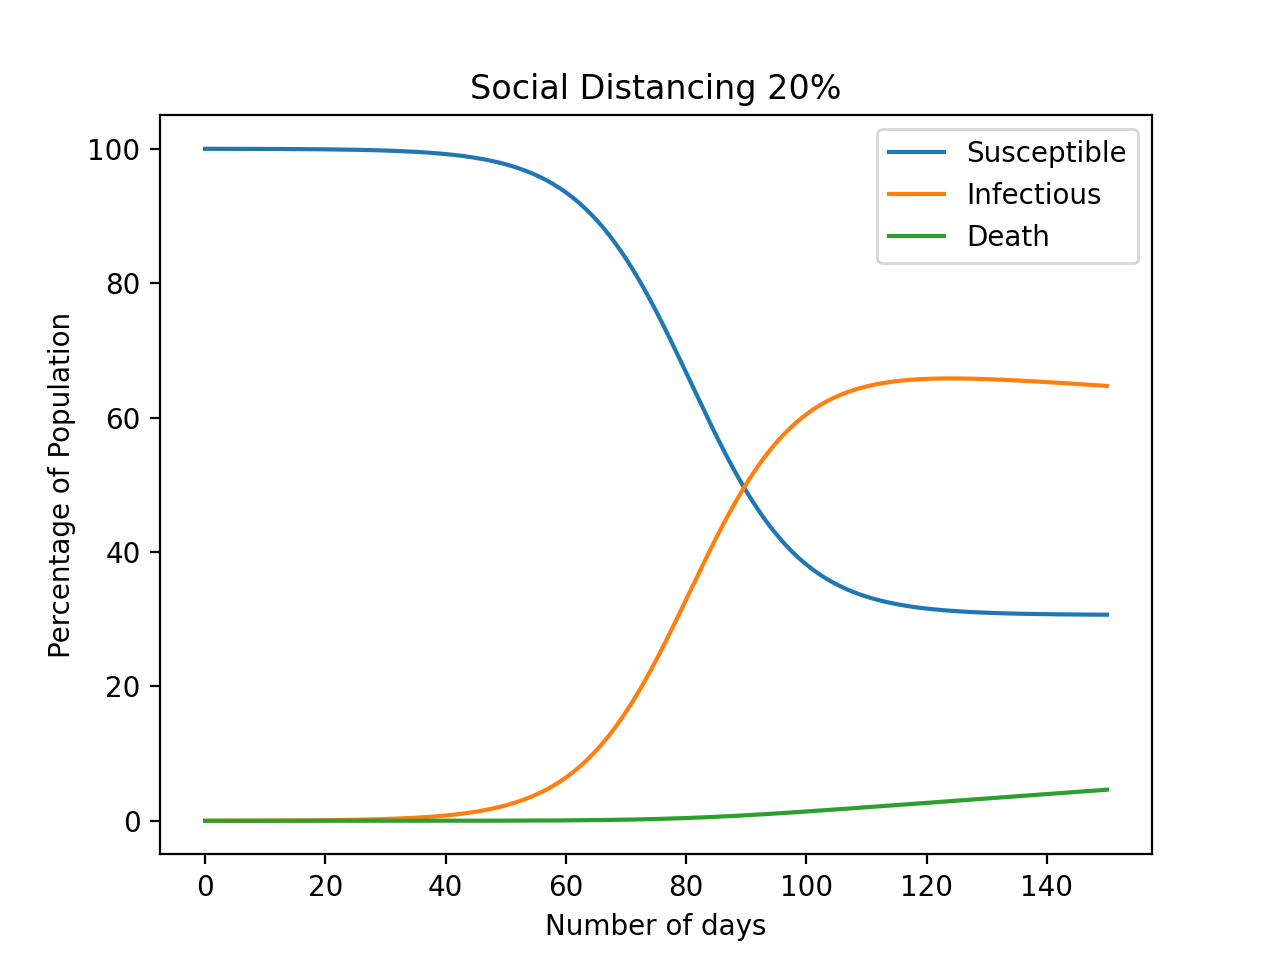
\includegraphics[width=90mm]{images/SISD/social_distance_20.png}
		\caption{SISD with $20\%$ social distancing}
	\end{figure}
	\clearpage
	\begin{figure}[h!]
		\centering
		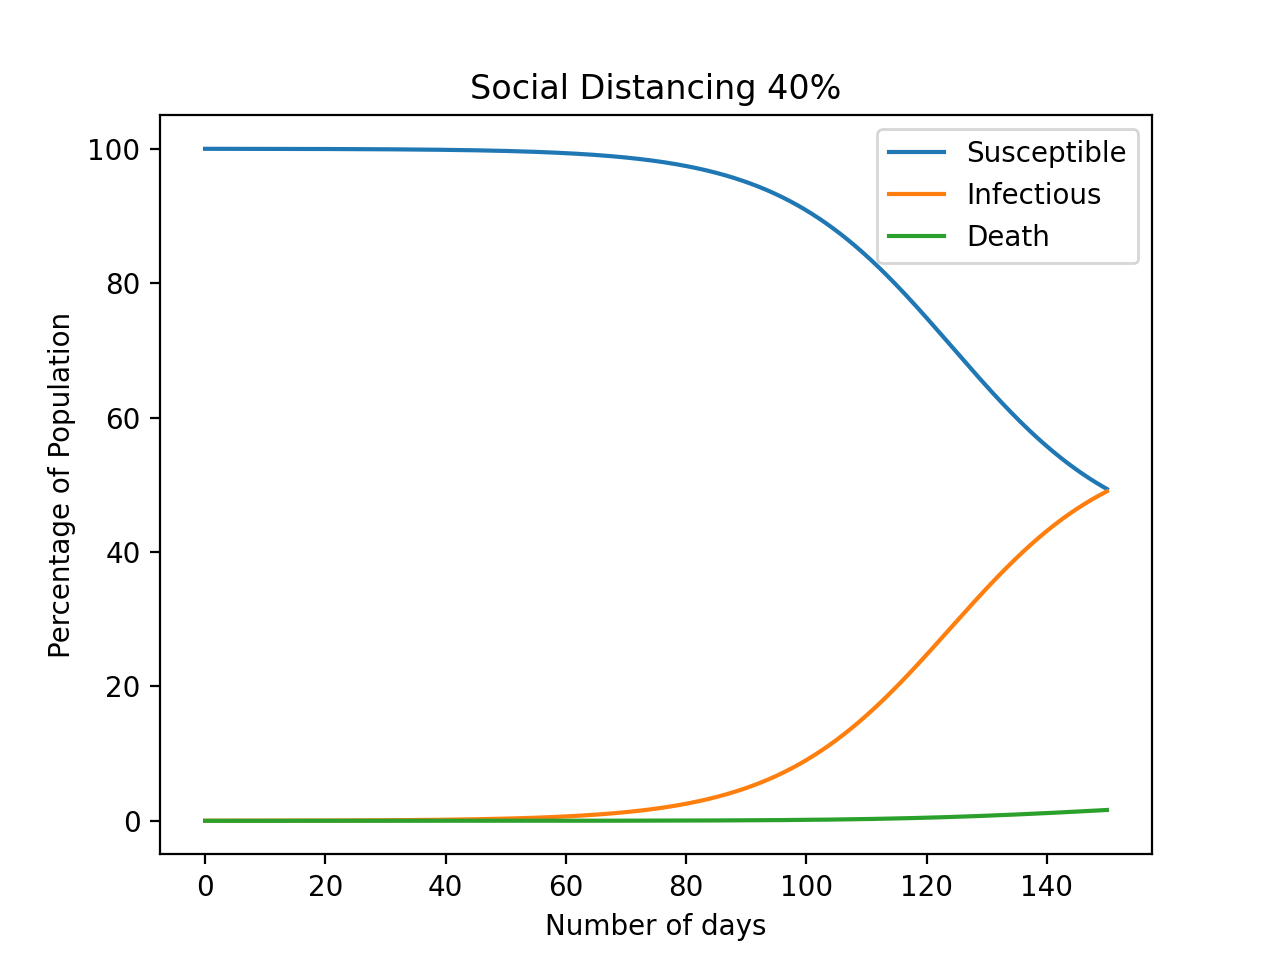
\includegraphics[width=90mm]{images/SISD/social_distance_40.png}
		\caption{SISD with $40\%$ social distancing}
	\end{figure}
	\begin{figure}[h!]
		\centering
		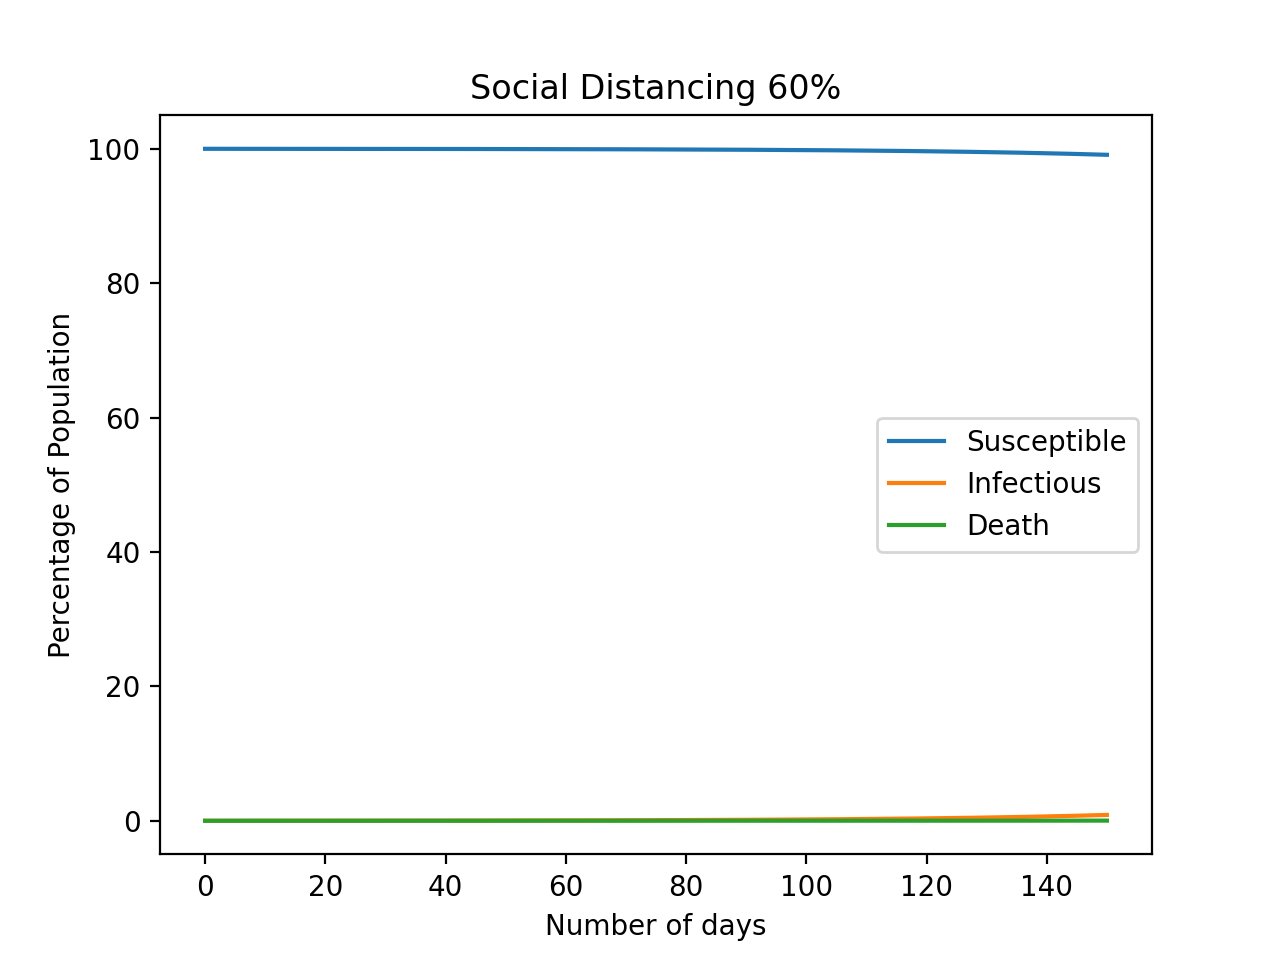
\includegraphics[width=90mm]{images/SISD/social_distance_60.png}
		\caption{SISD with $60\%$ social distancing}
	\end{figure}
	\clearpage
	\begin{figure}[h!]
		\centering
		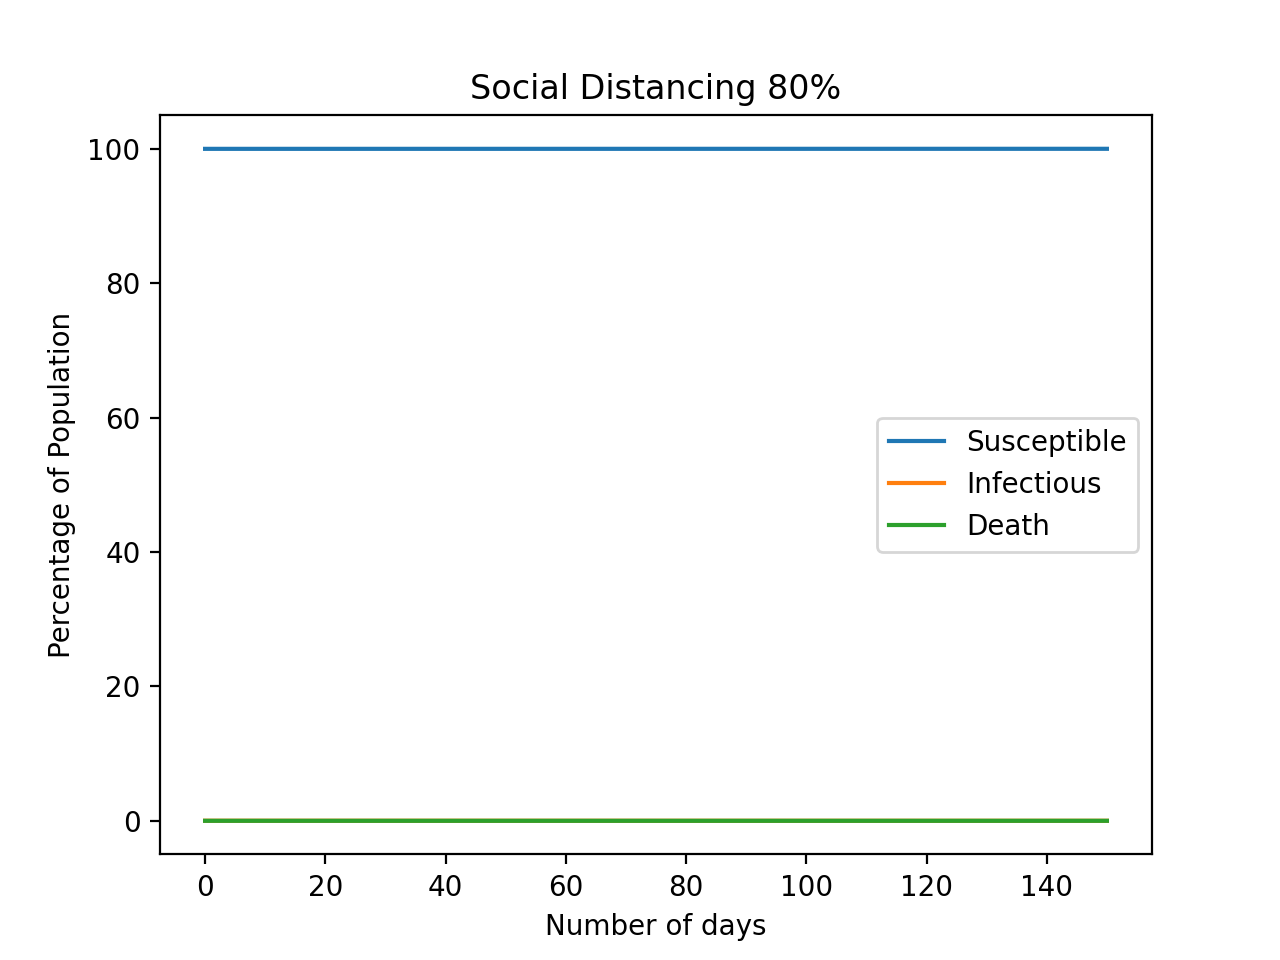
\includegraphics[width=90mm]{images/SISD/social_distance_80.png}
		\caption{SISD with $80\%$ social distancing}
	\end{figure}

	\subsection{SIXD}
	\begin{figure}[h!]
		\centering
		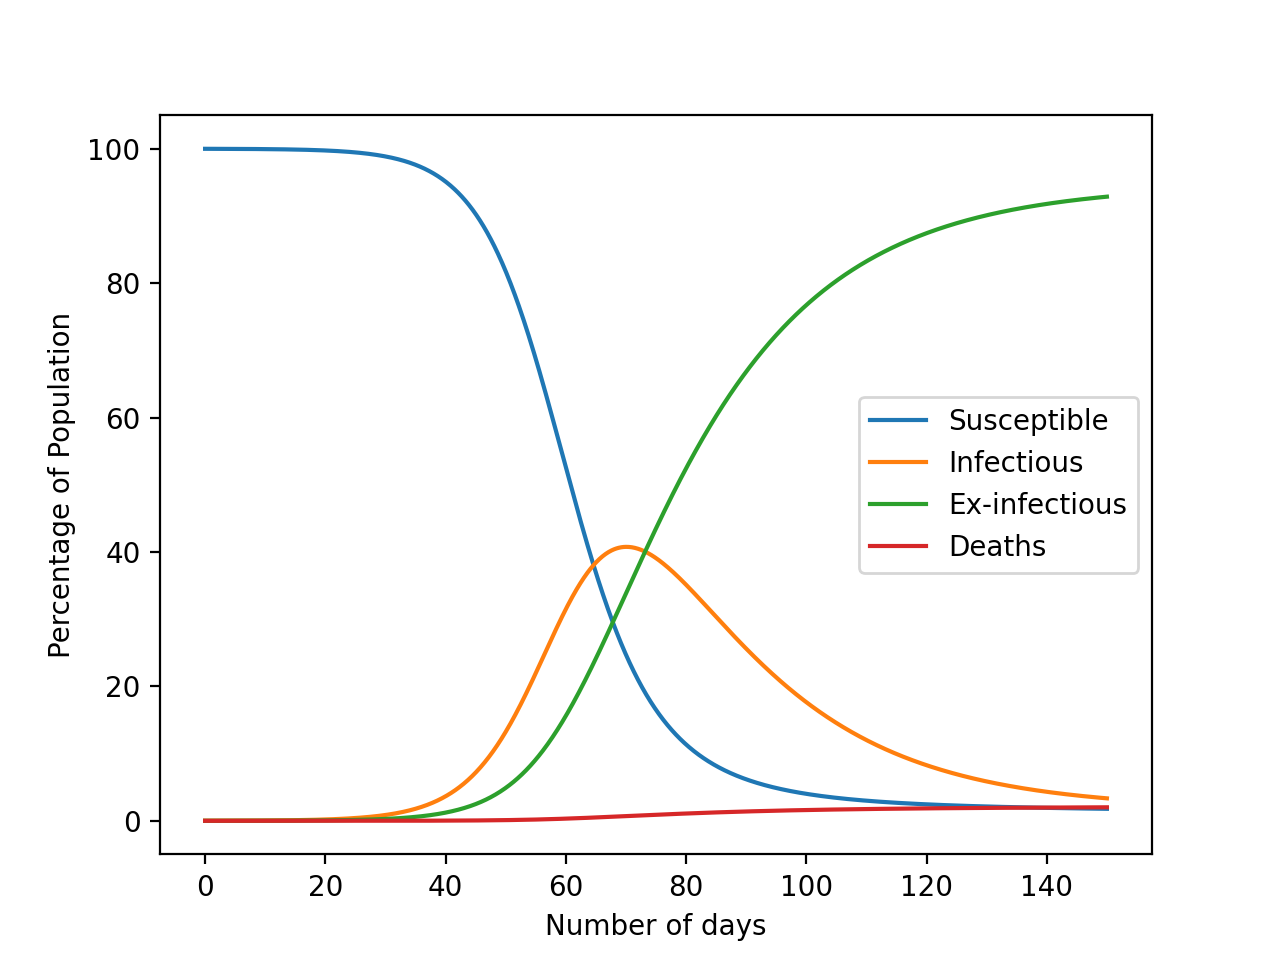
\includegraphics[width=90mm]{images/SIXD/standard.png}
		\caption{SIXD}
	\end{figure}
	\clearpage
	\begin{figure}[h!]
		\centering
		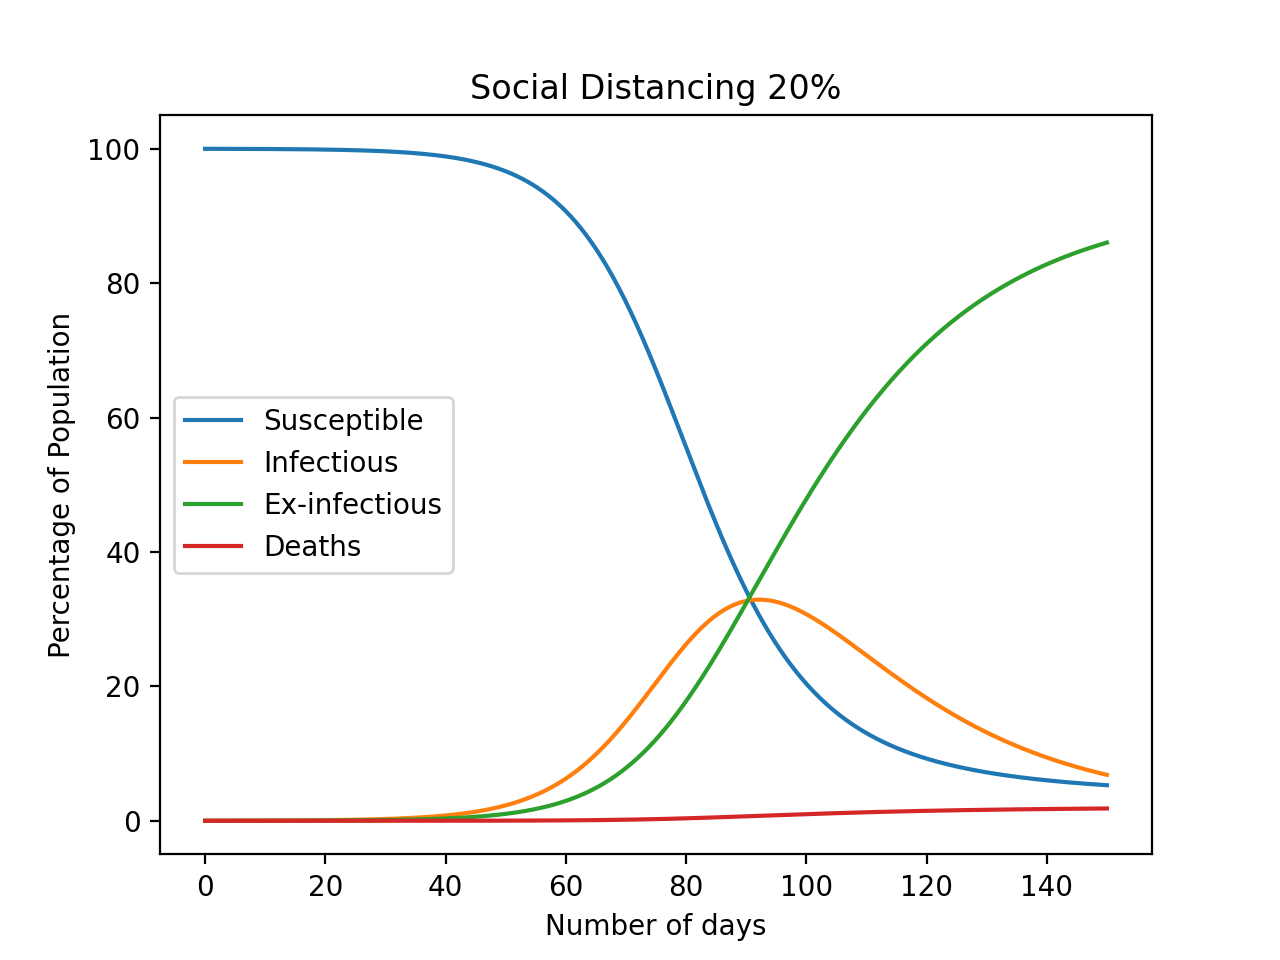
\includegraphics[width=90mm]{images/SIXD/social_distance_20.png}
		\caption{SIXD with $20\%$ social distancing}
	\end{figure}
	\begin{figure}[h!]
		\centering
		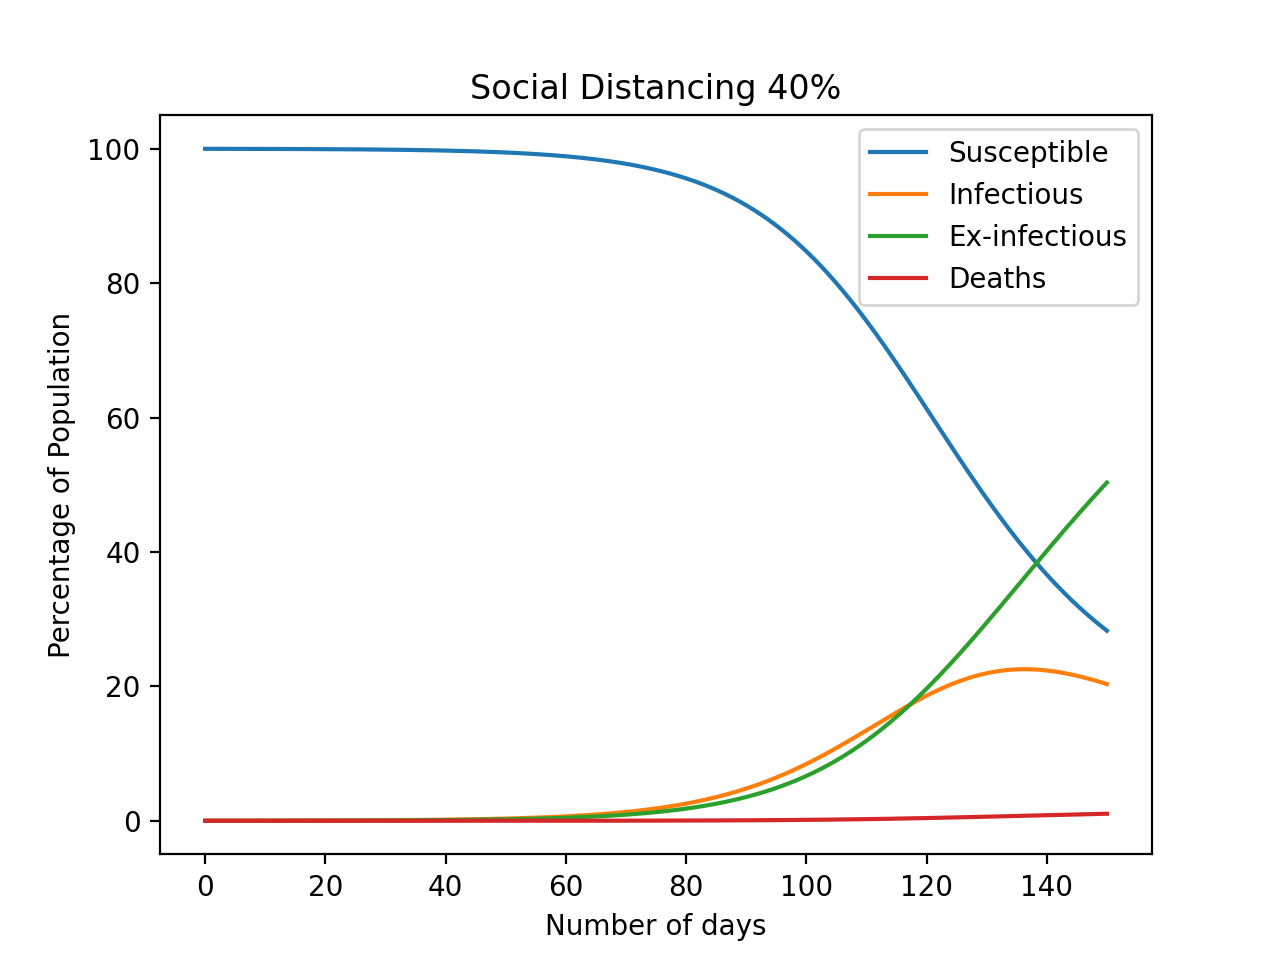
\includegraphics[width=90mm]{images/SIXD/social_distance_40.png}
		\caption{SIXD with $40\%$ social distancing}
	\end{figure}
	\clearpage
	\begin{figure}[h!]
		\centering
		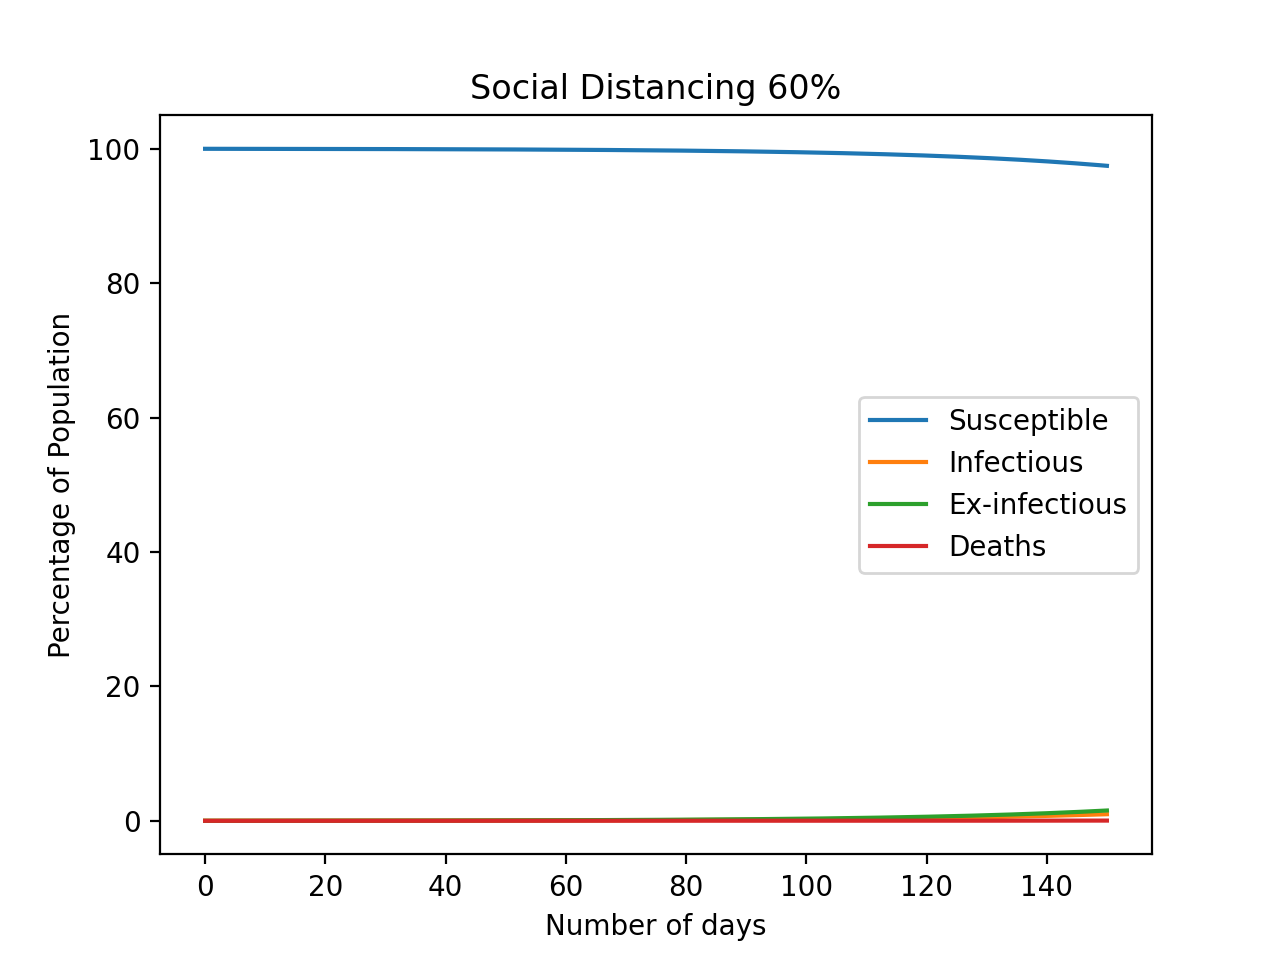
\includegraphics[width=90mm]{images/SIXD/social_distance_60.png}
		\caption{SIXD with $60\%$ social distancing}
	\end{figure}
	\begin{figure}[h!]
		\centering
		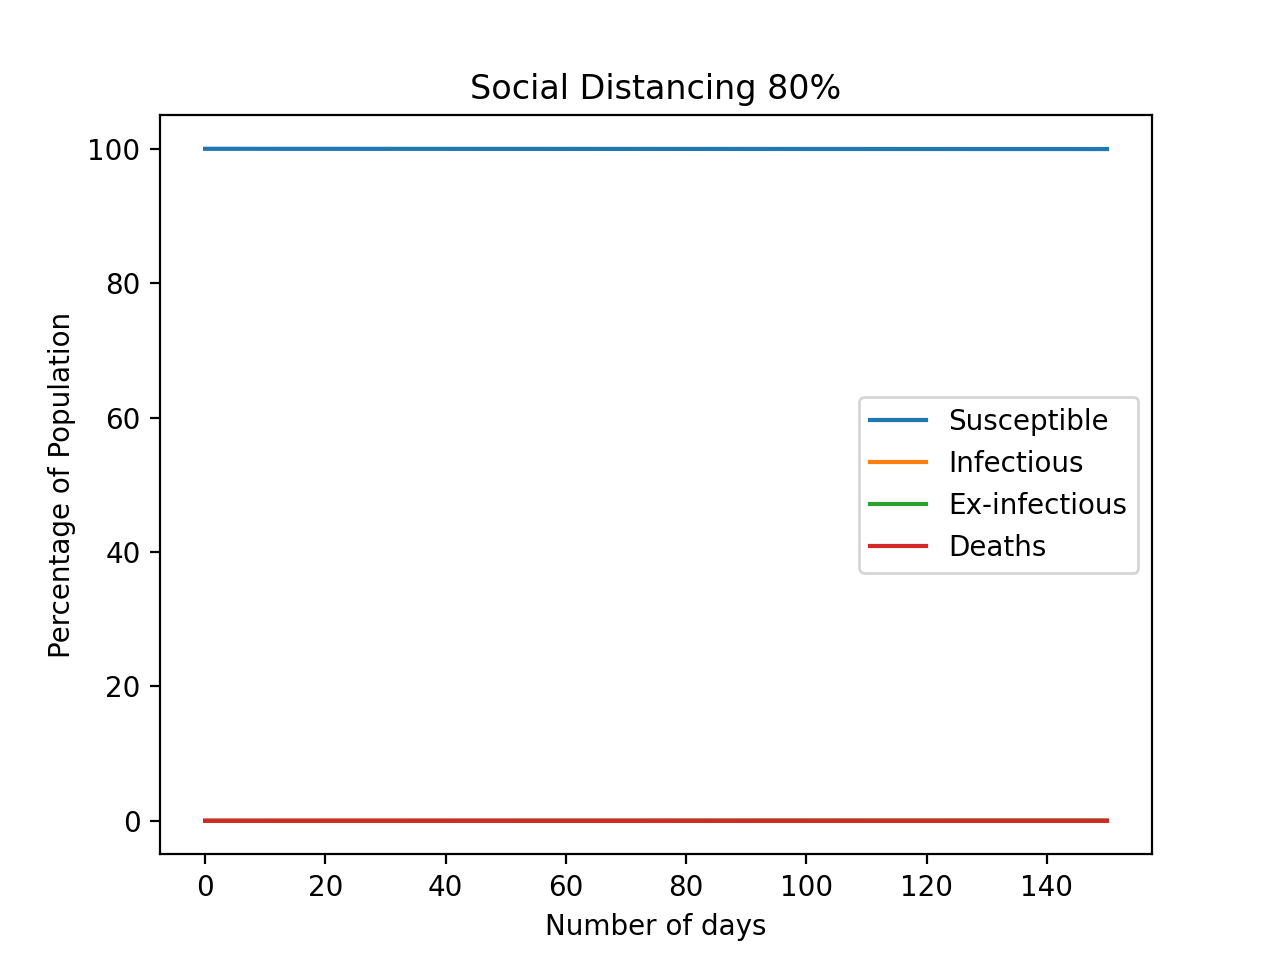
\includegraphics[width=90mm]{images/SIXD/social_distance_80.png}
		\caption{SIXD with $80\%$ social distancing}
	\end{figure}
	\clearpage

	\subsection{Comparision with SIR}
	\begin{figure}[h!]
		\centering
		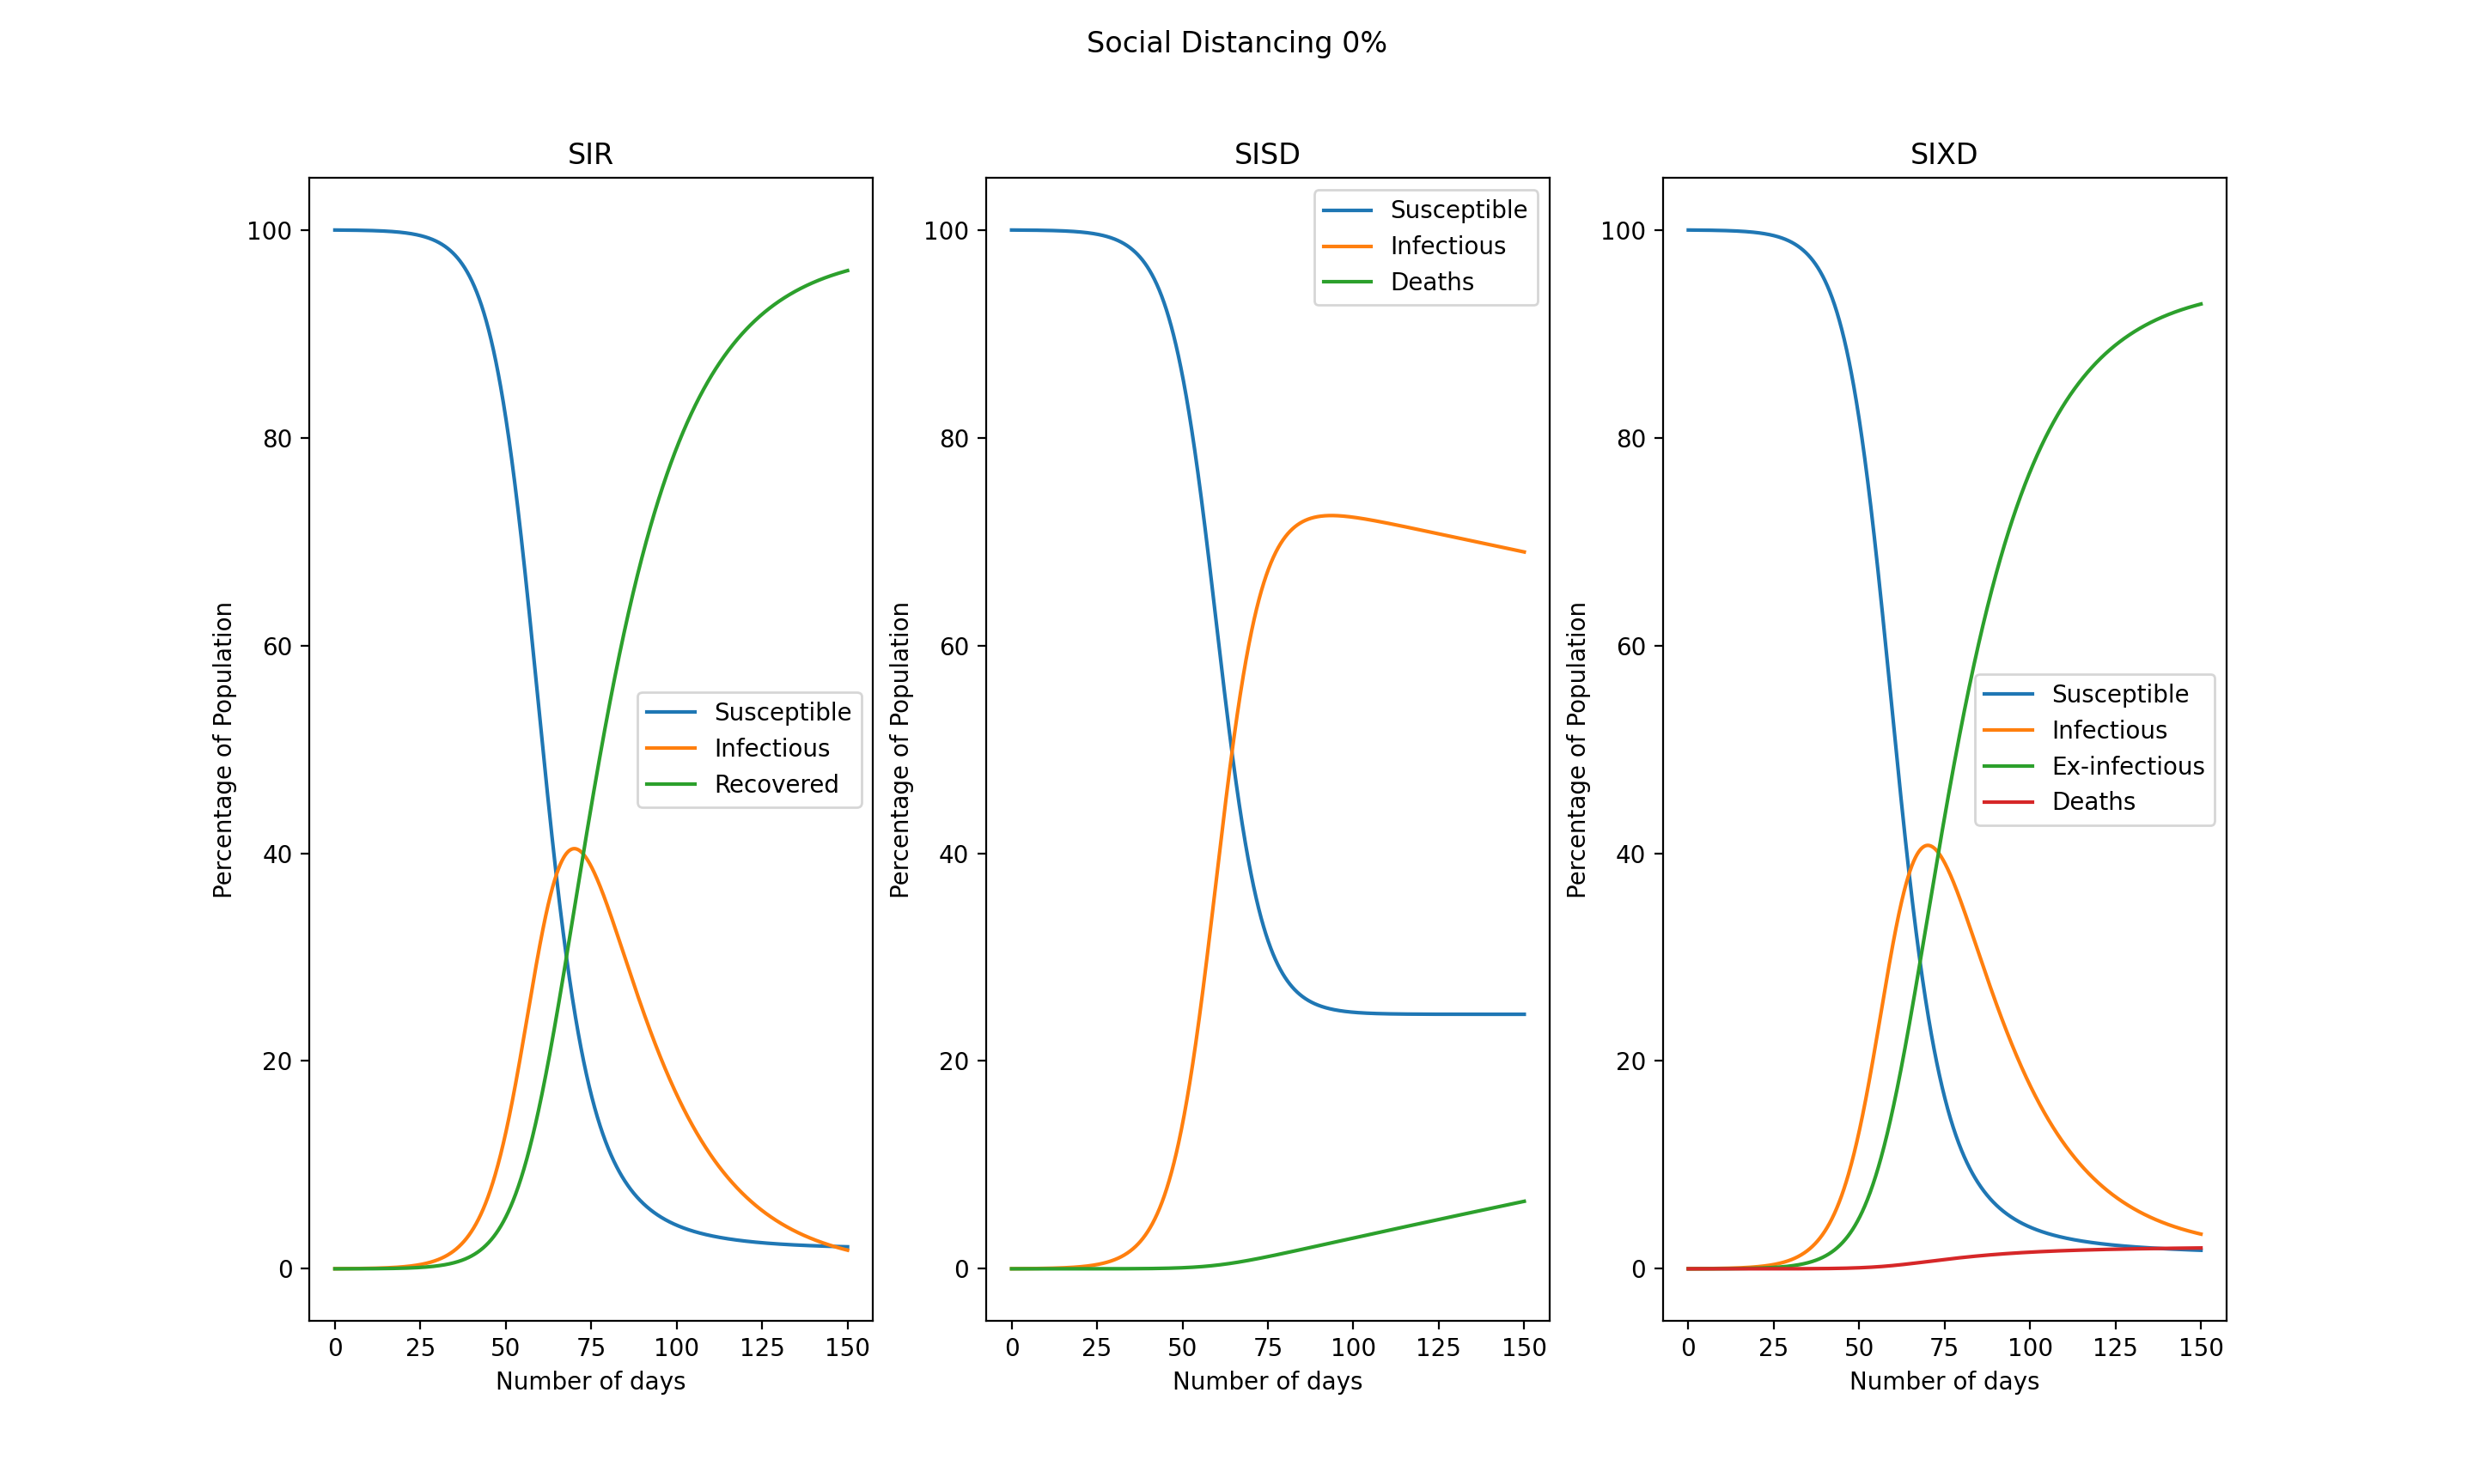
\includegraphics[width=90mm]{images/SIR/standard.png}
		\caption{Comparision of SIR, SISD, SIXD}
	\end{figure}
	\begin{figure}[h!]
		\centering
		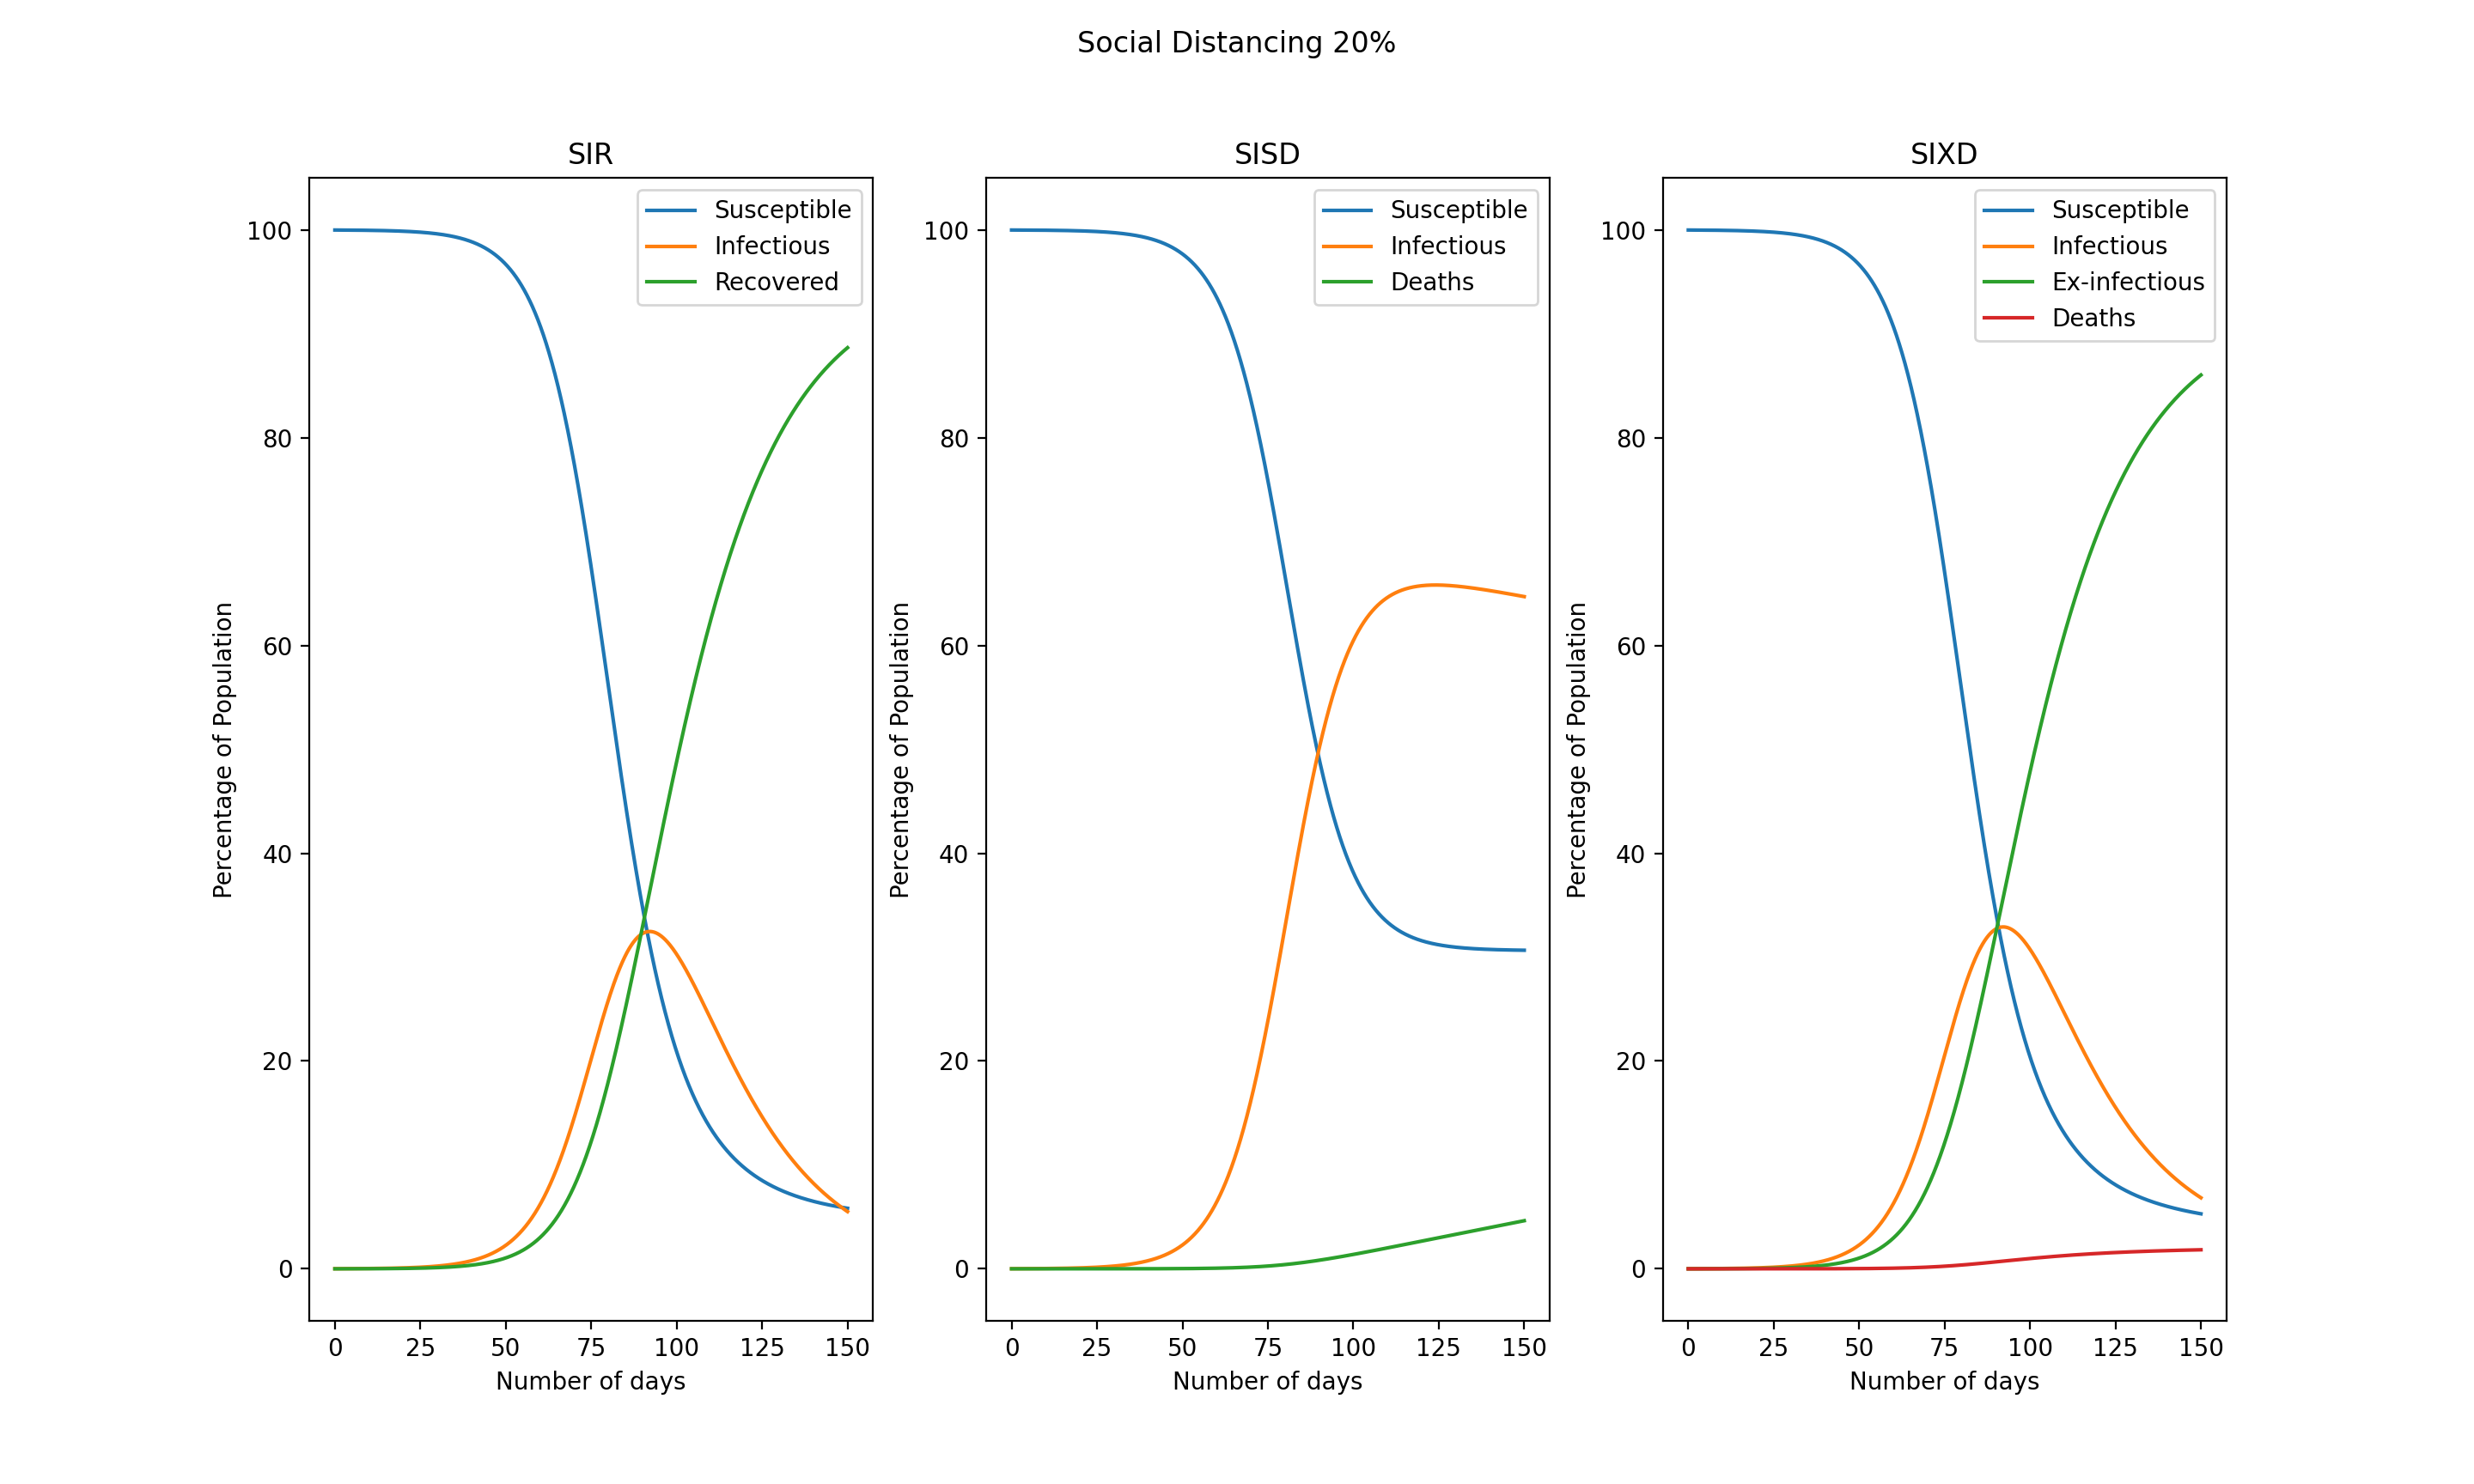
\includegraphics[width=90mm]{images/SIR/social_distance_20.png}
		\caption{Comparision of SIR, SISD, SIXD with $20\%$ social distancing}
	\end{figure}
	\clearpage
	\begin{figure}[h!]
		\centering
		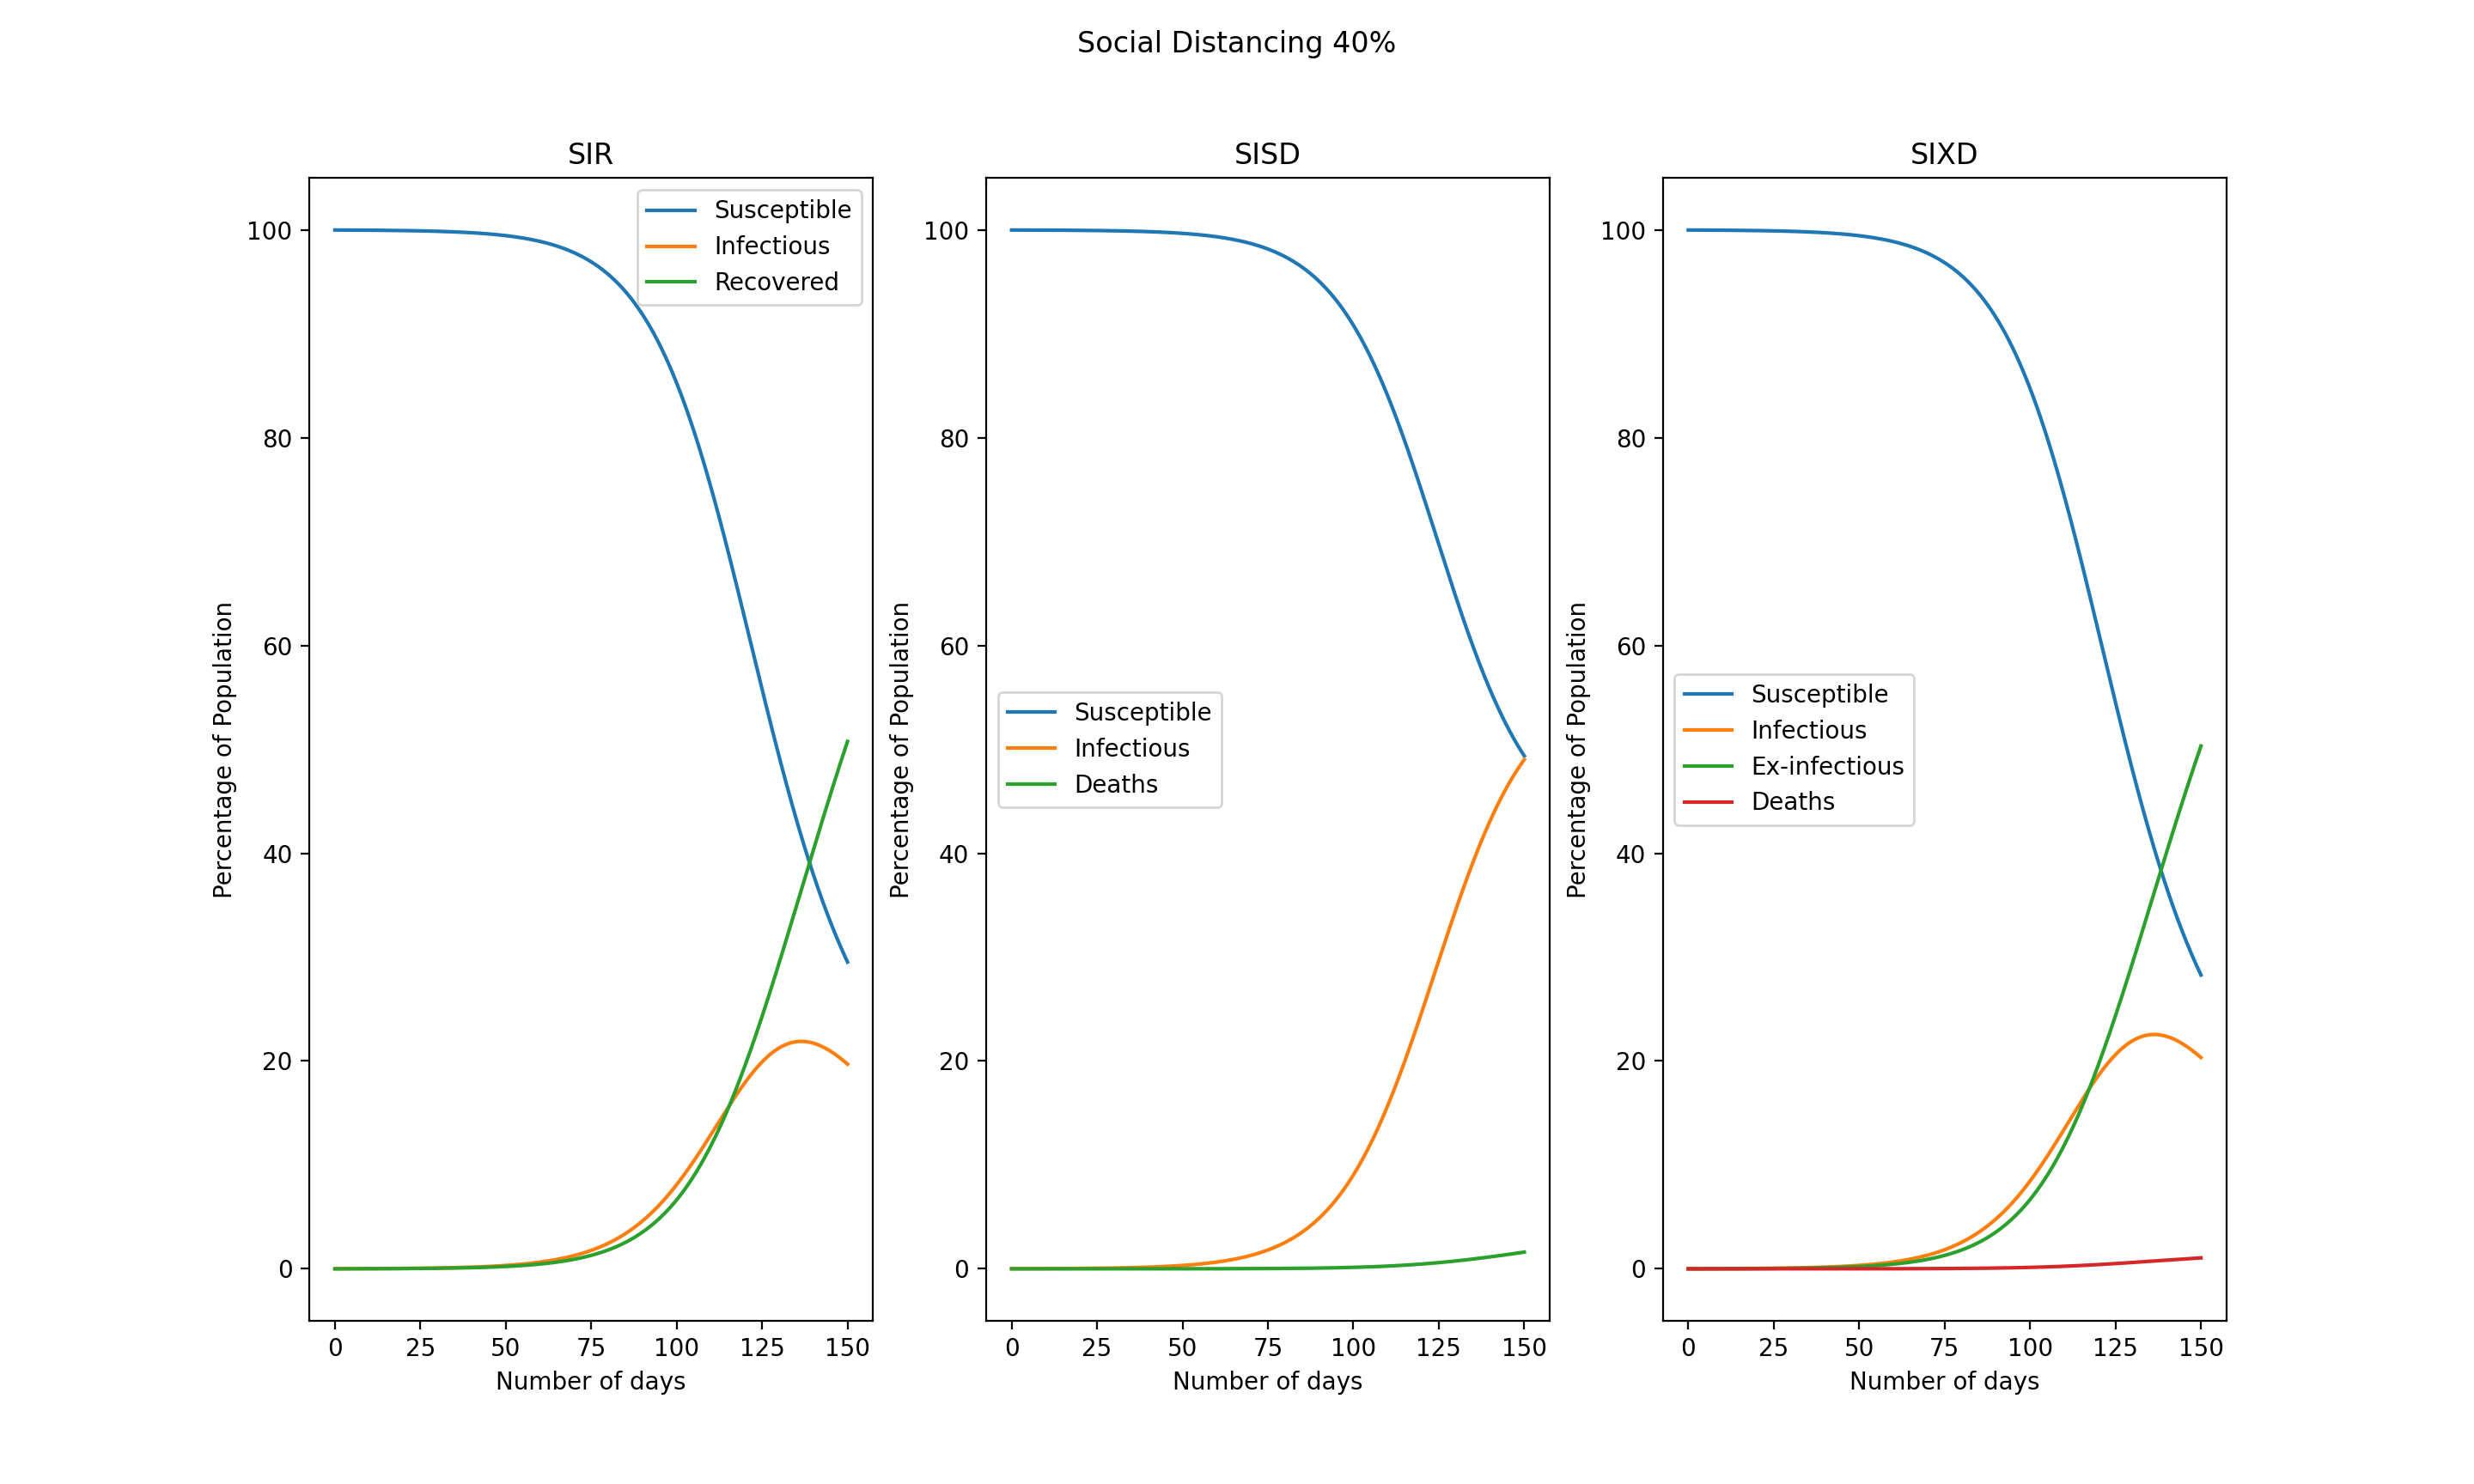
\includegraphics[width=90mm]{images/SIR/social_distance_40.png}
		\caption{Comparision of SIR, SISD, SIXD with $40\%$ social distancing}
	\end{figure}
	\begin{figure}[h!]
		\centering
		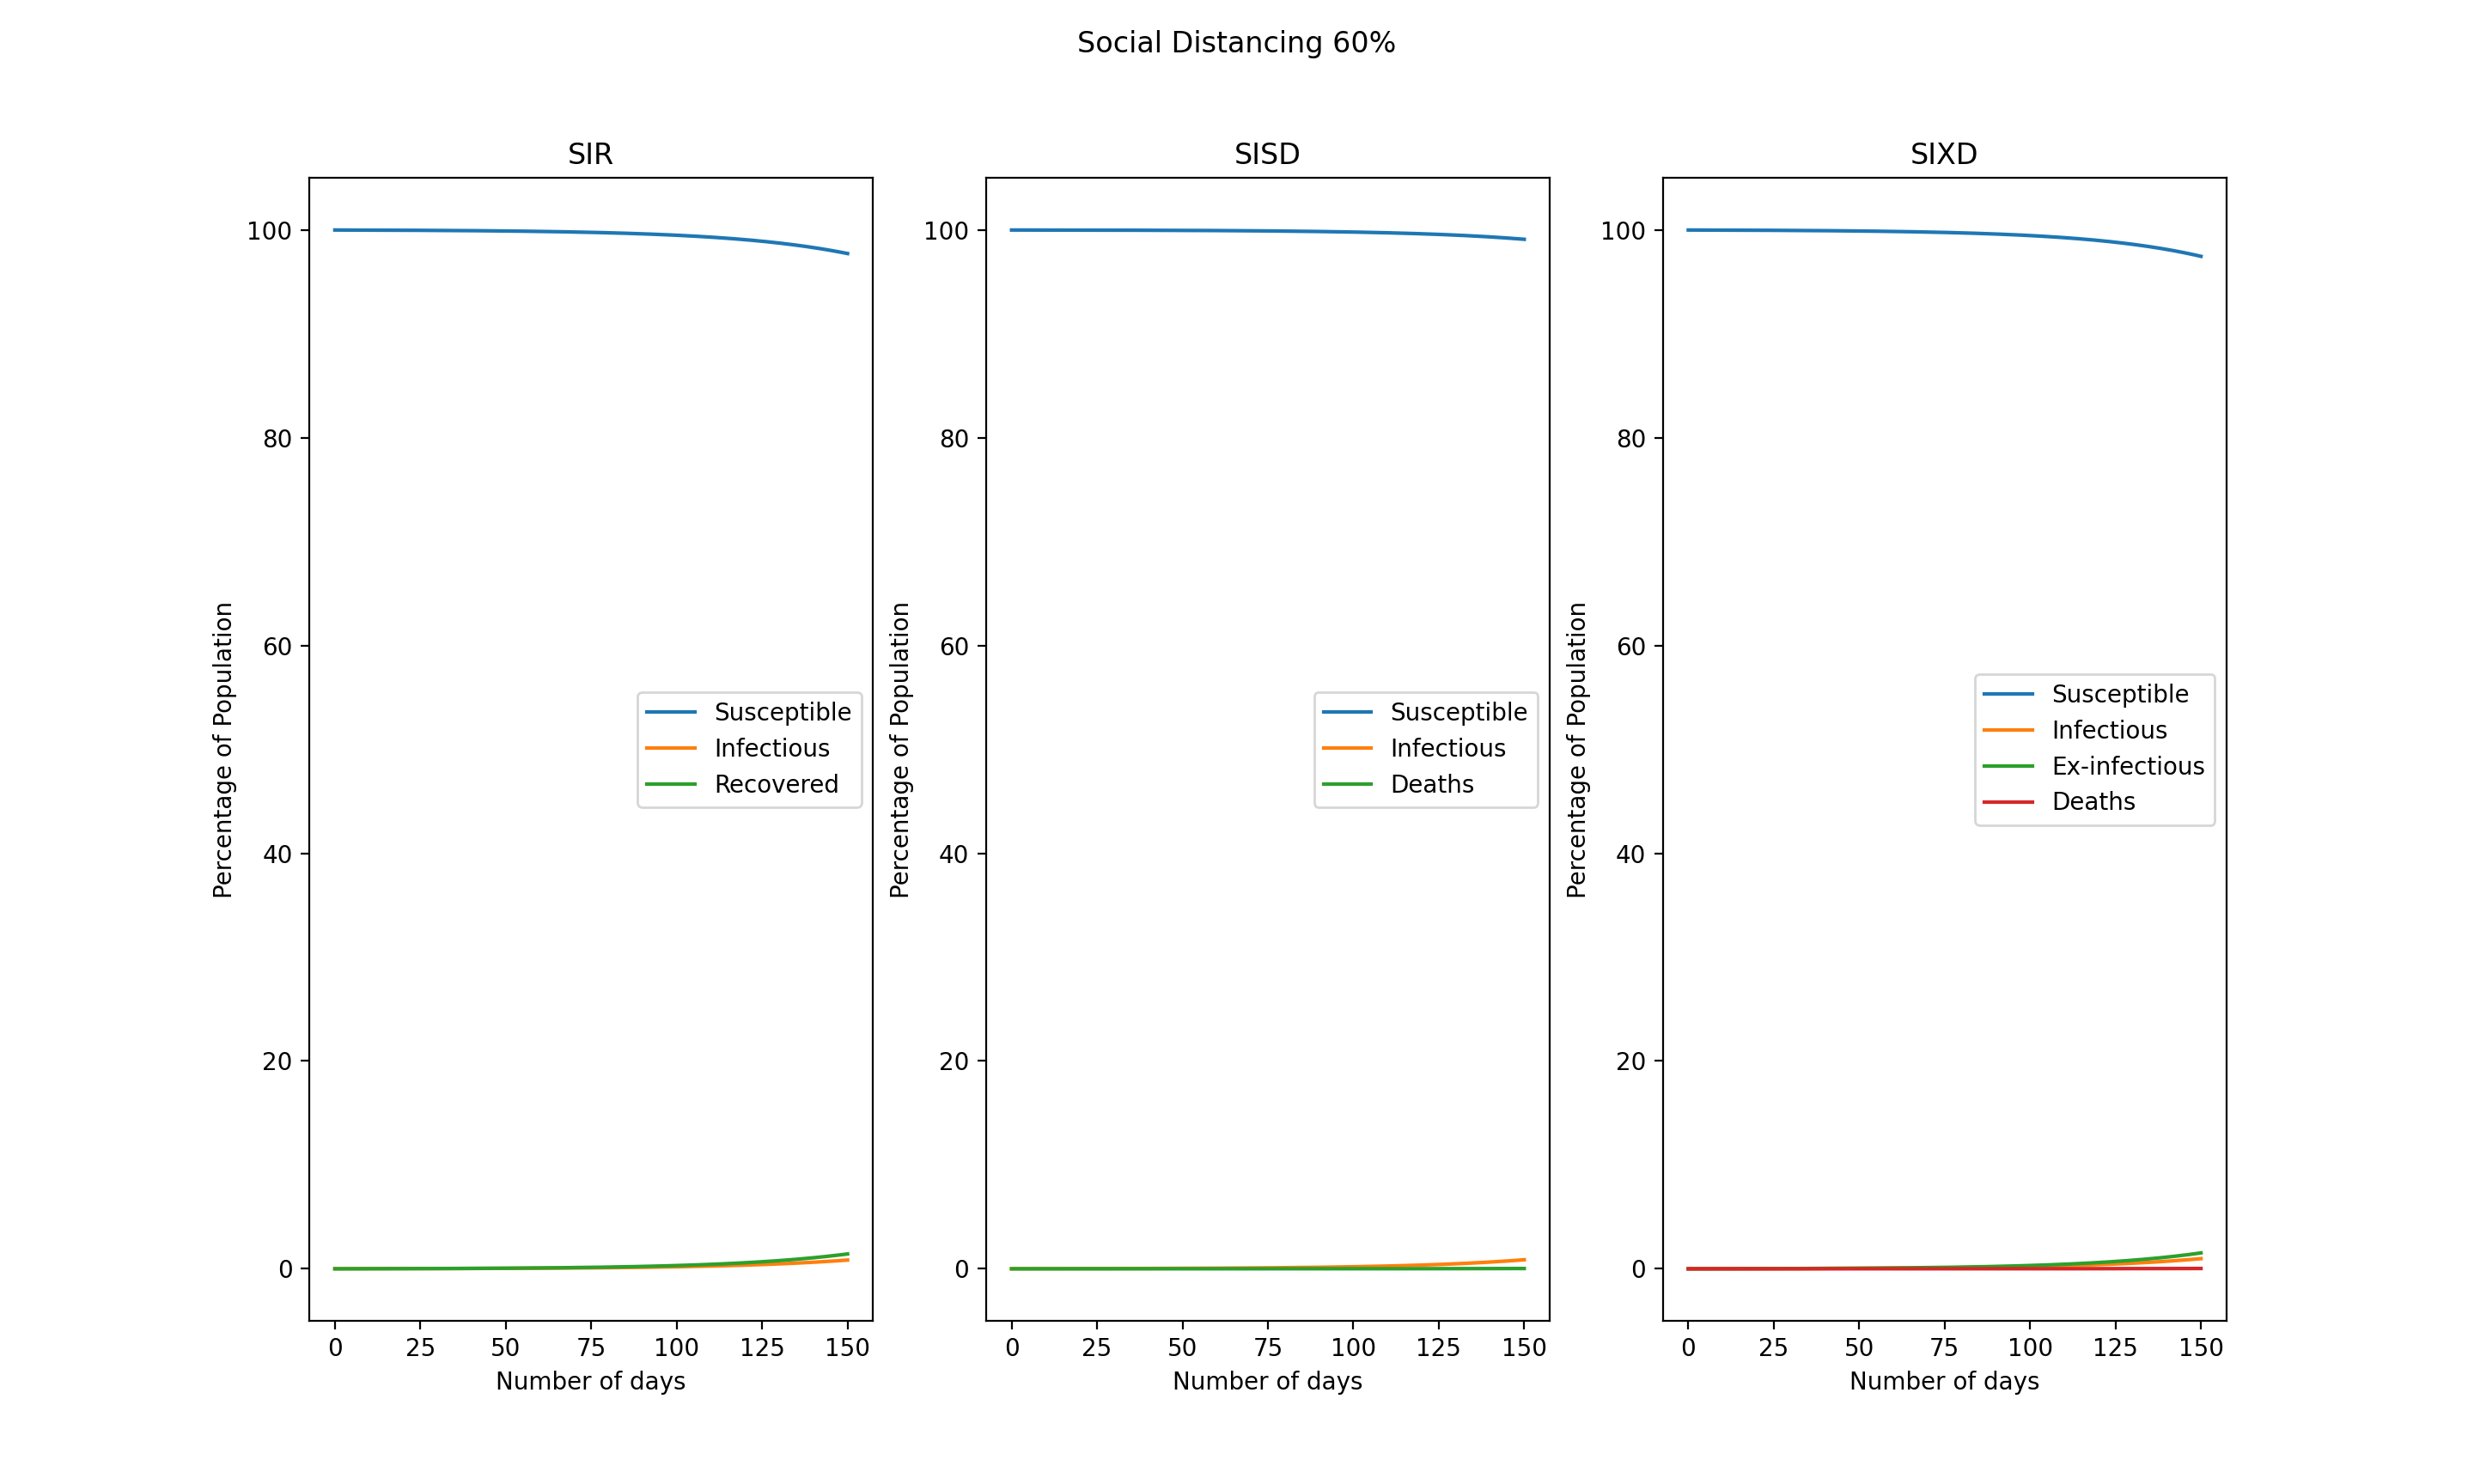
\includegraphics[width=90mm]{images/SIR/social_distance_60.png}
		\caption{Comparision of SIR, SISD, SIXD with $60\%$ social distancing}
	\end{figure}
	\clearpage
	\begin{figure}[h!]
		\centering
		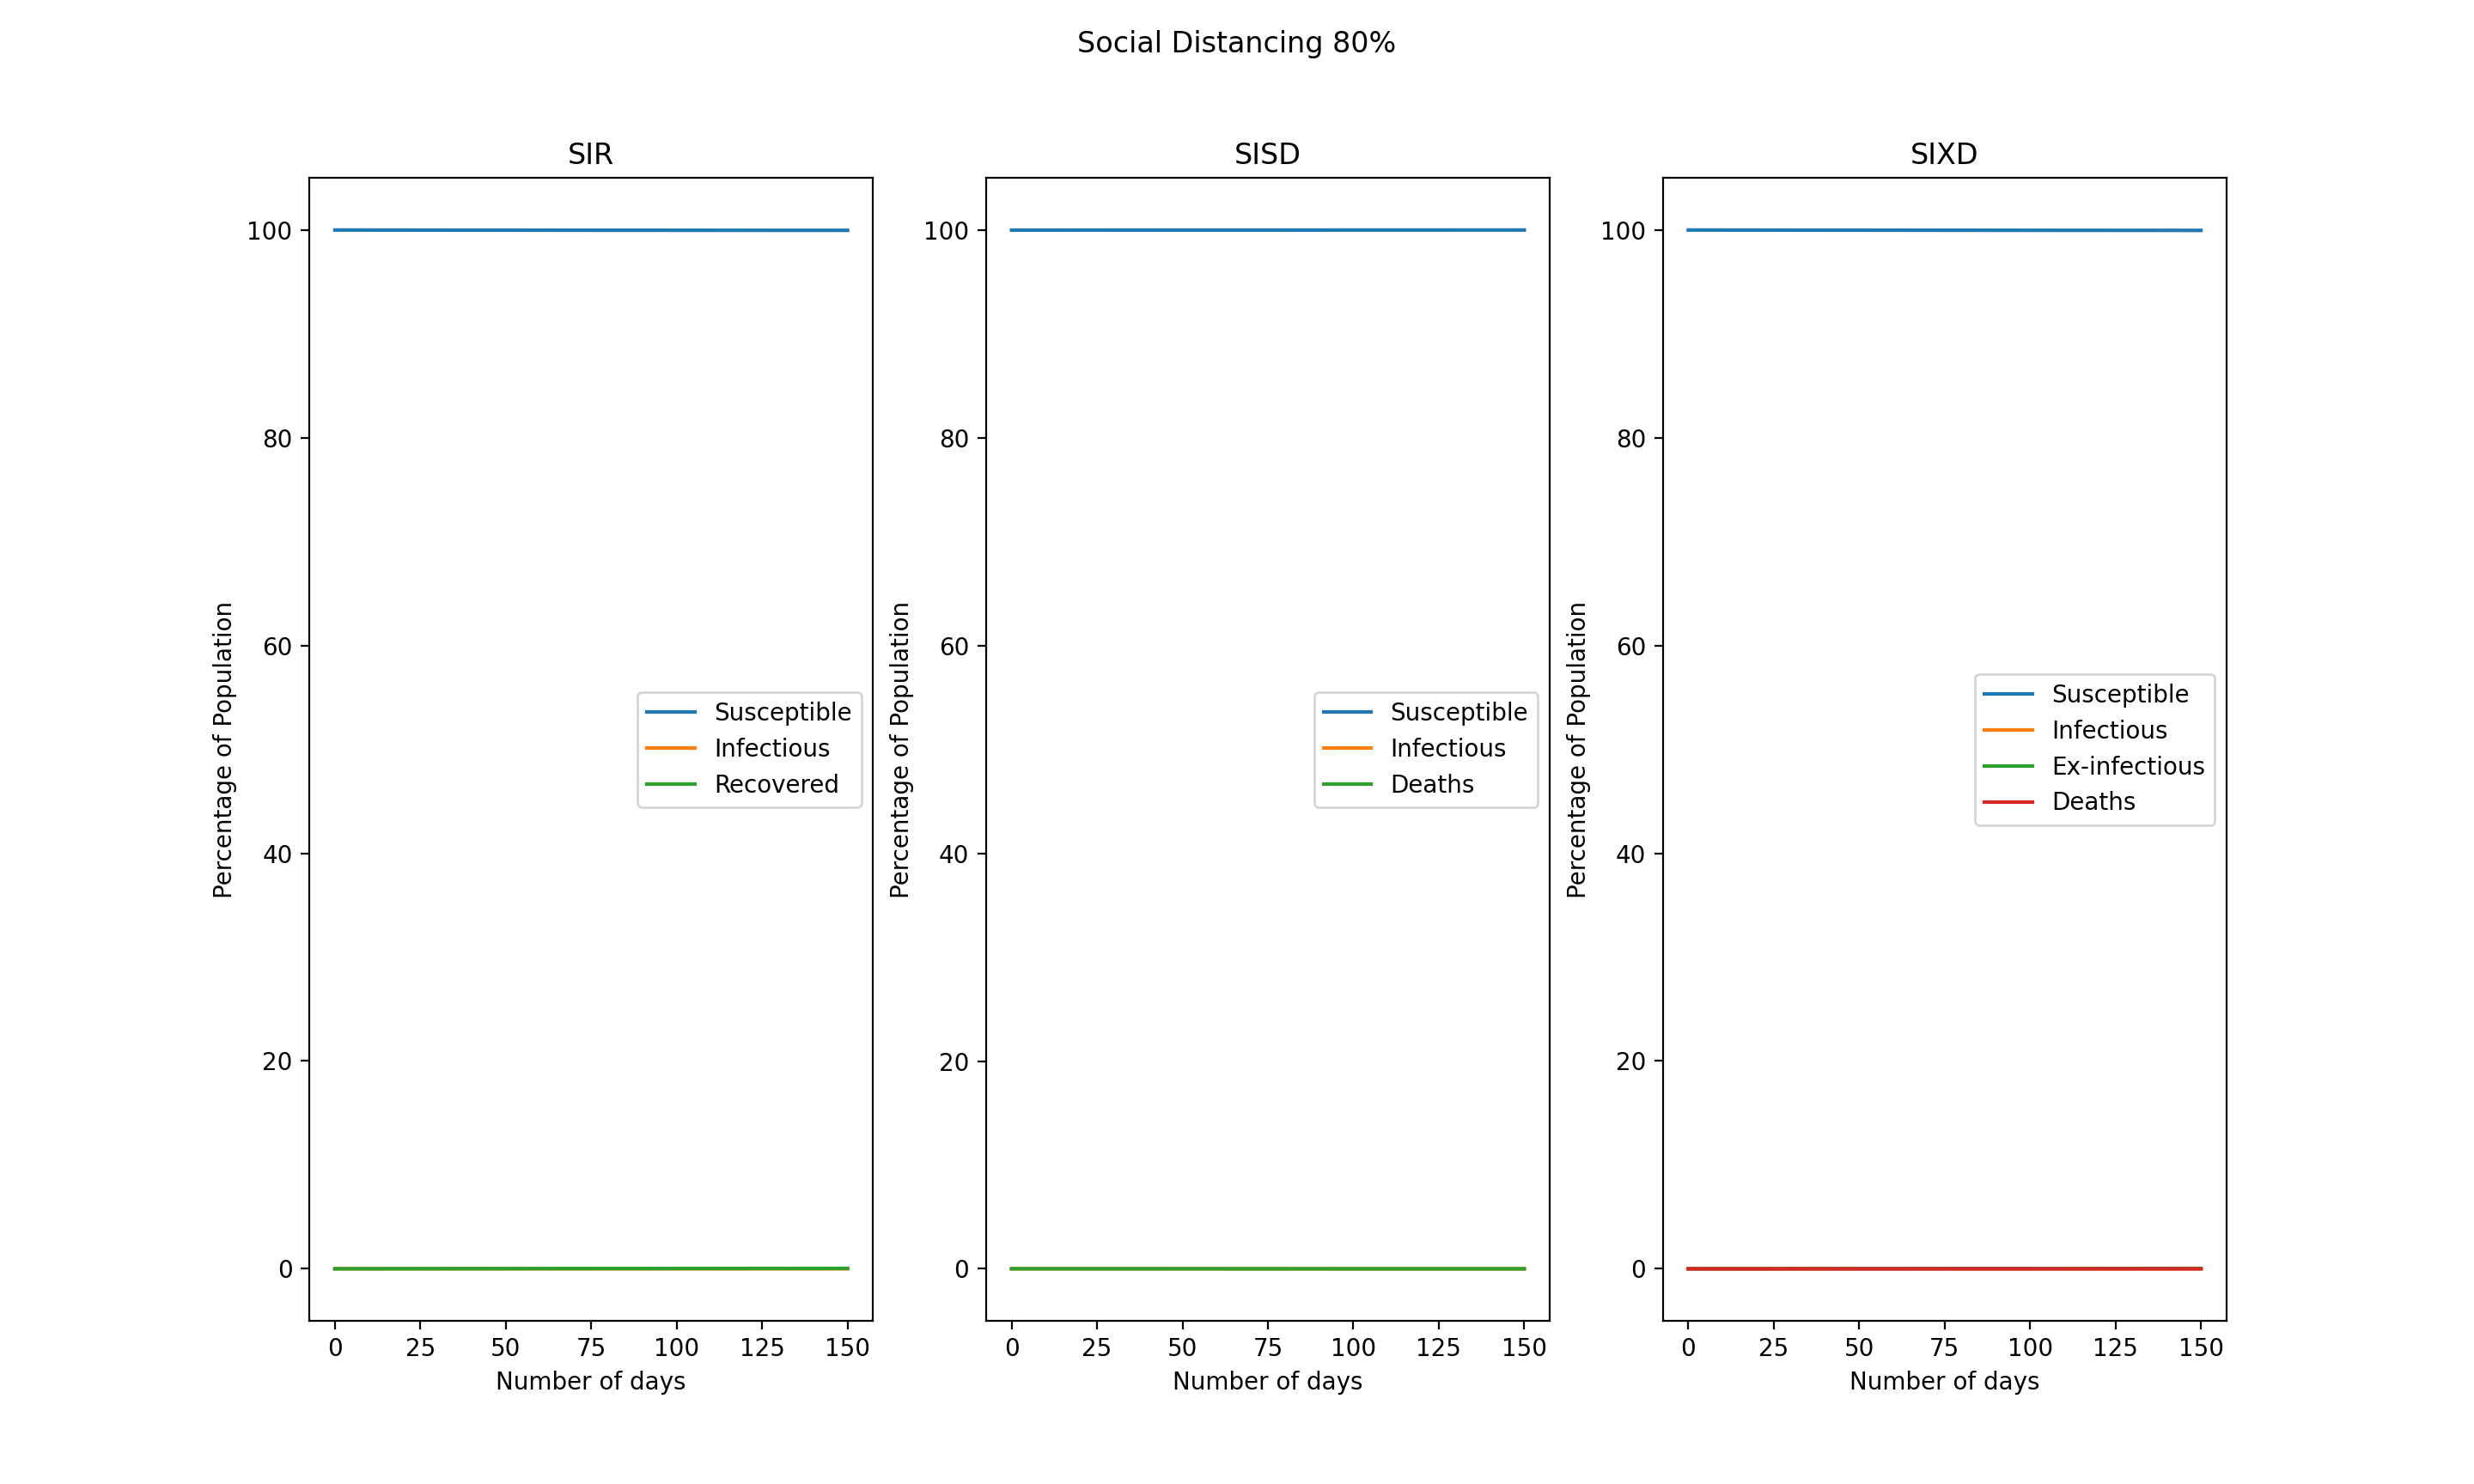
\includegraphics[width=90mm]{images/SIR/social_distance_80.png}
		\caption{Comparision of SIR, SISD, SIXD with $80\%$ social distancing}
	\end{figure}


	\section{Observations}
	We chose to simulate for 150 days as well documented data is available for us to compare the effectivness of our models. Following observations were drawn from the simulation:
	\begin{itemize}
		\item All models highlight the importance of social distancing. Also, we showed how at $80\%$ of social distancing, disease was completely cutoff from spreading. 
		\item SIR and SIXD models behave very similary. This implies that the re-generation of virus has no significant effect in the short term.
		\item More social distancing tends to lessen the height of the infectious curve thereby curbing the pressure on medical infrastructure.
		\item Our models also show that social distancing tends to delay the onset of the infection peak which gives time for the government to take appropriate healthcare decisions.
		\item SIXD model like SIR model does predict the peak of the curve approximately which occurs at around 100 days with certain social distancing measures.[6]
		\item Since in most cases more than $50\%$ social distancing is tough to implement, the models present an economic vs healthcare tradeoff. Stricter social distancing parameters would lessen the peak of the curve but would delay it's onset. Onset delay means we've to observe the social distancing measures for a long time which will affect the economic activities. On the other hand, sharp peak might put immense pressure on the healthcare system.
	\end{itemize}

	\section{Contribution}
	Our unique contribution to this project is attributed to the fact that we are using SIS to model the COVID-19 outbreak. We had extensively researched the possibility of reoccurence of the virus. Our intuition behind this approach was simple. COVID-19 is just another flu, like the common cold. Hence, it is very much possible that a person may not develop the required immunity against the virus just like the common cold. Besides this, we also factored in the concept of social distancing for our SISD and SIXD models as explained above. 
	Moving on to perhaps our most important contribution to the project is the parameter $\theta$ in the SIXD model. $\theta$ stands for re-activation rate. Simply put, it's the factor which helps in determining the probability of a recovered individual getting tested positive again. \textit{One of the biggest accomplishments of this project is to calculate $\theta$ which came out to be 0.00085.}

	\section{References}
	\begin{enumerate}
		\item \href{https://royalsocietypublishing.org/doi/10.1098/rspa.1927.0118}{A contribution to the mathematical theory of epidemics by William Ogilvy Kermack and A. G. McKendrick}
		\item \href{https://github.com/midas-network/COVID-19}{MIDAS Research Networks}
		\item \href{https://www.cdc.go.kr/cdc_eng/}{Korea Centers for Disease Control and Prevention}
		\item \href{https://www.who.int/bulletin/online_first/20-255158.pdf}{WHO Report: Epidemic situation and forecasting of COVID-19}
		\item \href{https://www.who.int/news-room/commentaries/detail/immunity-passports-in-the-context-of-covid-19}{WHO Report: Immunit Passports in context of COVID-19}
		\item \href{https://www.worldometers.info/coronavirus/country/italy/}{Active cases of COVID-19 in Italy}{}
	\end{enumerate}

\end{document}
